% !TEX TS-program = pdflatex
% !TEX encoding = UTF-8 Unicode

% This is a simple template for a LaTeX document using the "article" class.
% See "book", "report", "letter" for other types of document.

\documentclass[11pt]{article} % use larger type; default would be 10pt

\usepackage[utf8]{inputenc} % set input encoding (not needed with XeLaTeX)


%%% Examples of Article customizations
% These packages are optional, depending whether you want the features they provide.
% See the LaTeX Companion or other references for full information.

%%% PAGE DIMENSIONS
\usepackage{geometry} % to change the page dimensions
\geometry{a4paper} % or letterpaper (US) or a5paper or....
% \geometry{margin=2in} % for example, change the margins to 2 inches all round
\geometry{landscape} % set up the page for landscape
%   read geometry.pdf for detailed page layout information

\usepackage{graphicx} % support the \includegraphics command and options
\usepackage[outdir=./]{epstopdf}

% \usepackage[parfill]{parskip} % Activate to begin paragraphs with an empty line rather than an indent

%%% PACKAGES
\usepackage{booktabs} % for much better looking tables
\usepackage{array} % for better arrays (eg matrices) in maths
\usepackage{paralist} % very flexible & customisable lists (eg. enumerate/itemize, etc.)
\usepackage{verbatim} % adds environment for commenting out blocks of text & for better verbatim
\usepackage{subfig} % make it possible to include more than one captioned figure/table in a single float
% These packages are all incorporated in the memoir class to one degree or another...

%%% HEADERS & FOOTERS
\usepackage{fancyhdr} % This should be set AFTER setting up the page geometry
\pagestyle{fancy} % options: empty , plain , fancy
\renewcommand{\headrulewidth}{0pt} % customise the layout...
\lhead{}\chead{}\rhead{}
\lfoot{}\cfoot{\thepage}\rfoot{}

%%% SECTION TITLE APPEARANCE
\usepackage{sectsty}
\allsectionsfont{\sffamily\mdseries\upshape} % (See the fntguide.pdf for font help)
% (This matches ConTeXt defaults)

%%% ToC (table of contents) APPEARANCE
\usepackage[nottoc,notlof,notlot]{tocbibind} % Put the bibliography in the ToC
\usepackage[titles,subfigure]{tocloft} % Alter the style of the Table of Contents
\renewcommand{\cftsecfont}{\rmfamily\mdseries\upshape}
\renewcommand{\cftsecpagefont}{\rmfamily\mdseries\upshape} % No bold!

%%% END Article customizations

%%% The "real" document content comes below...
\title{graphes}
\date{} % Activate to display a given date or no date (if empty),
         % otherwise the current date is printed 

% TODO : restructurer ce qui est écrit par avance

\begin{document}
\maketitle


\begin{figure}[h!]
  \caption{Masse invariante $\gamma \gamma$ des photons reconstruits (mother = H).(données 'ZH/all events')}
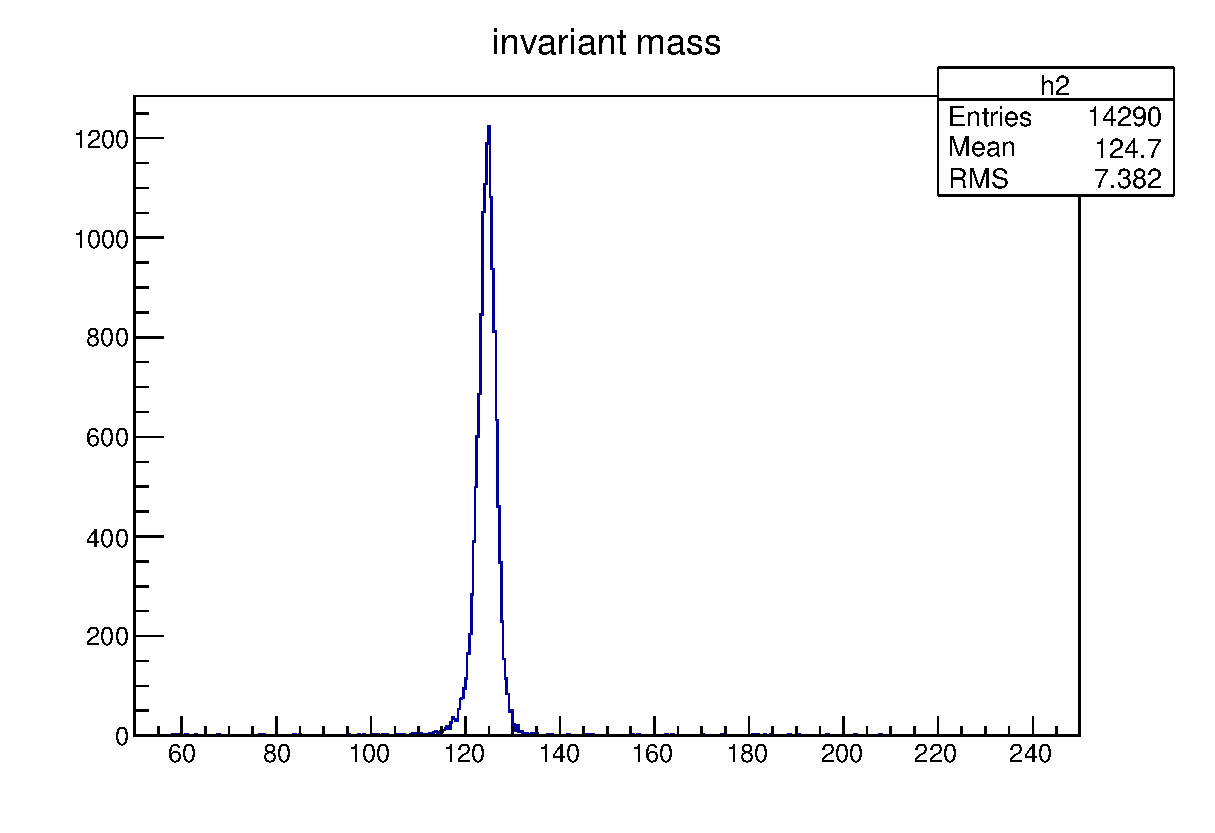
\includegraphics{../graphes/distrib_mgg_brute}
\end{figure}

\begin{figure}[h!]
  \caption{$M_{\gamma \gamma}$ cette fois basée sur les données 'true'.}
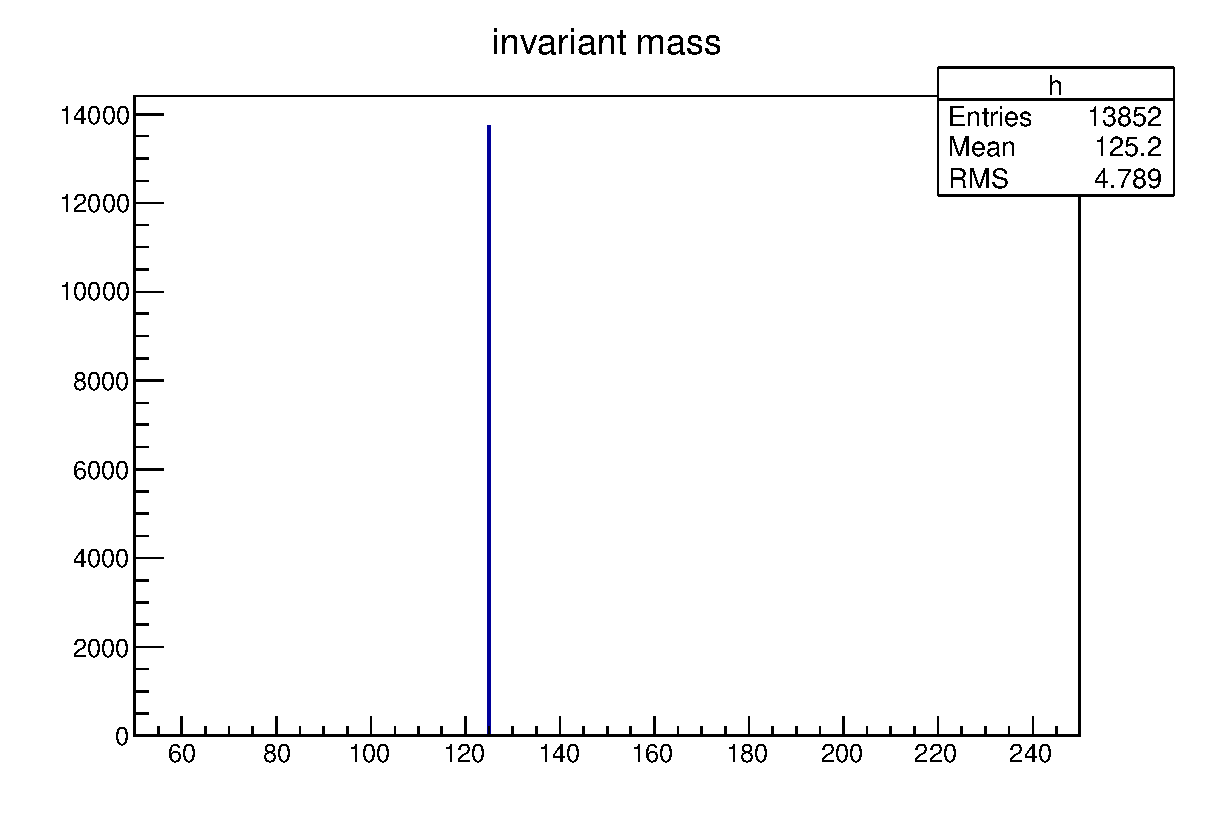
\includegraphics{../graphes/distrib_mgg_true_onlyH}
\end{figure}

\begin{figure}[h!]
  \caption{efficacité en fonction de $\eta$.}
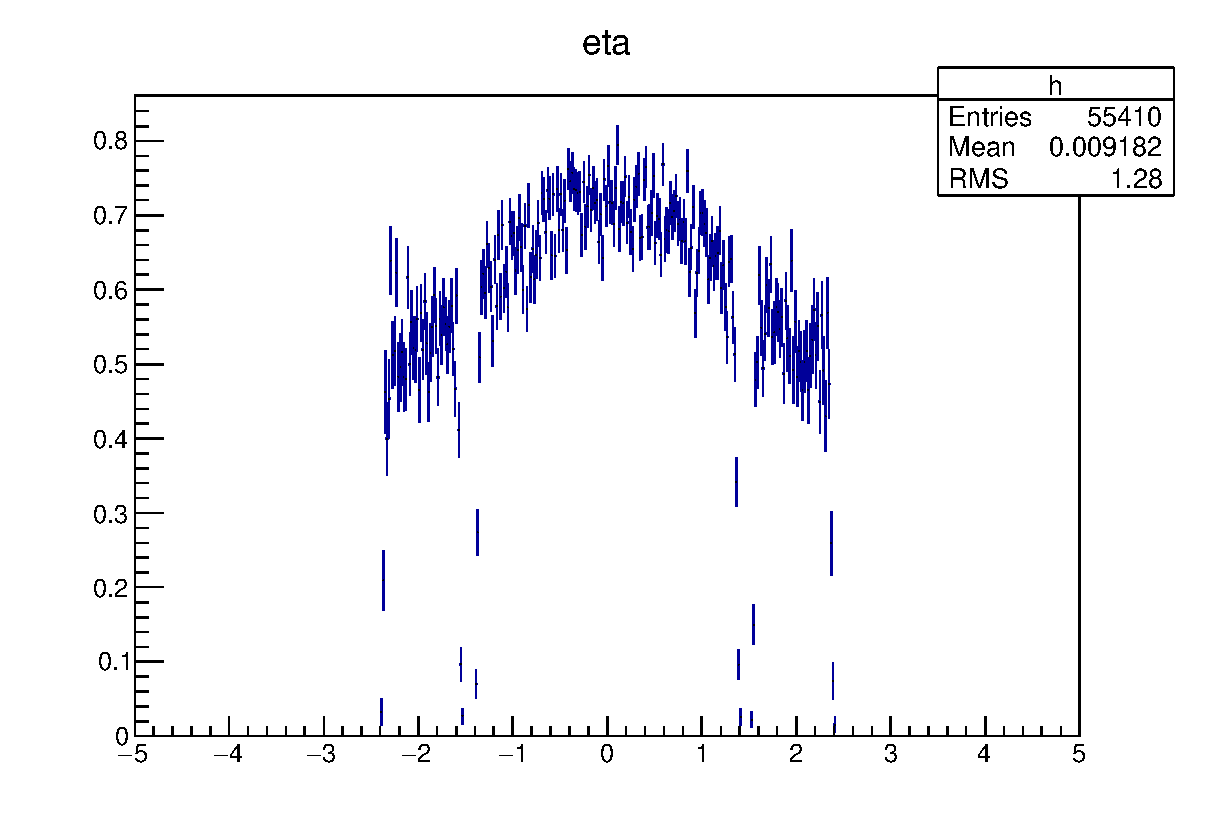
\includegraphics{../graphes/acceptance_eta_ph}
\end{figure}


\begin{figure}[h!]
  \caption{efficacité en fonction de $\phi$.}
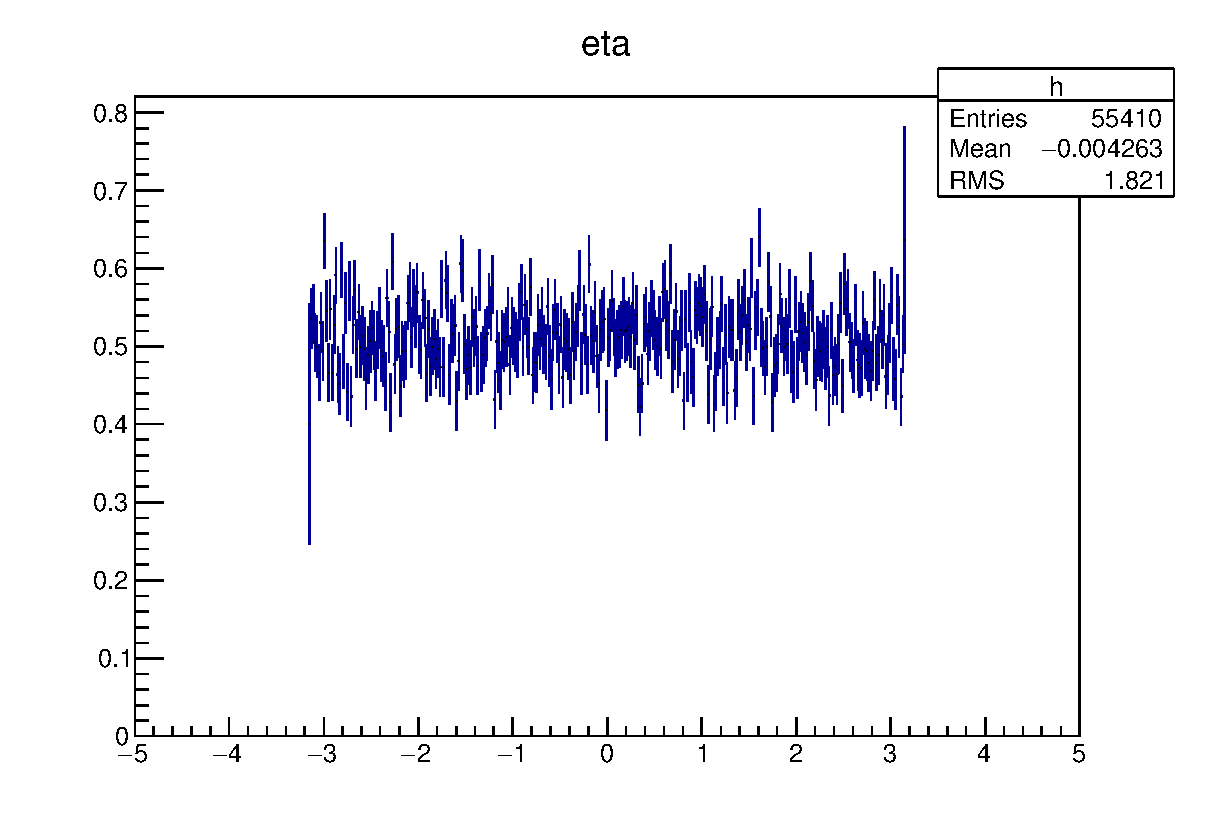
\includegraphics{../graphes/acceptance_phi_ph}
\end{figure}

\begin{figure}[h!]
  \caption{efficacité en fonction de $E_{T_\gamma}$ .}
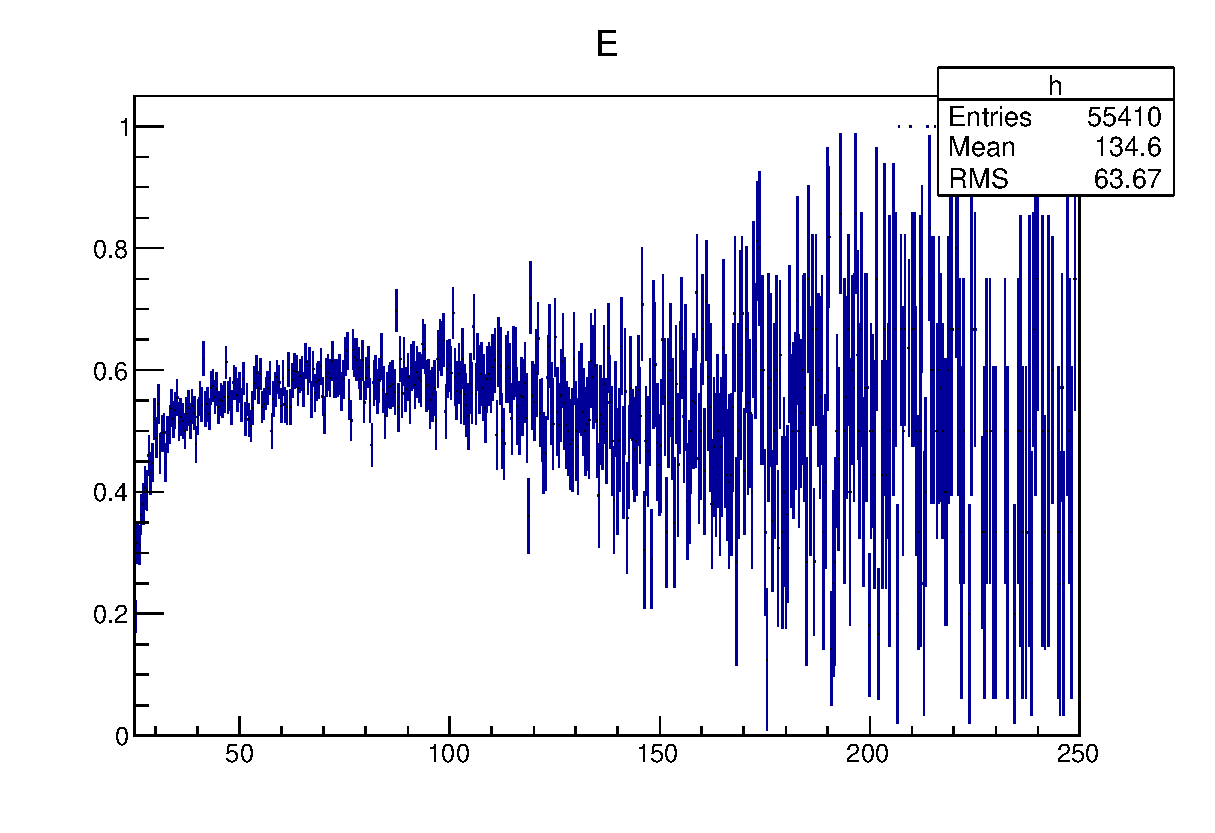
\includegraphics{../graphes/accep_et_raw}
\end{figure}

\begin{figure}[h!]
  \caption{distribution réelle des H en fonction de $\eta$ .}
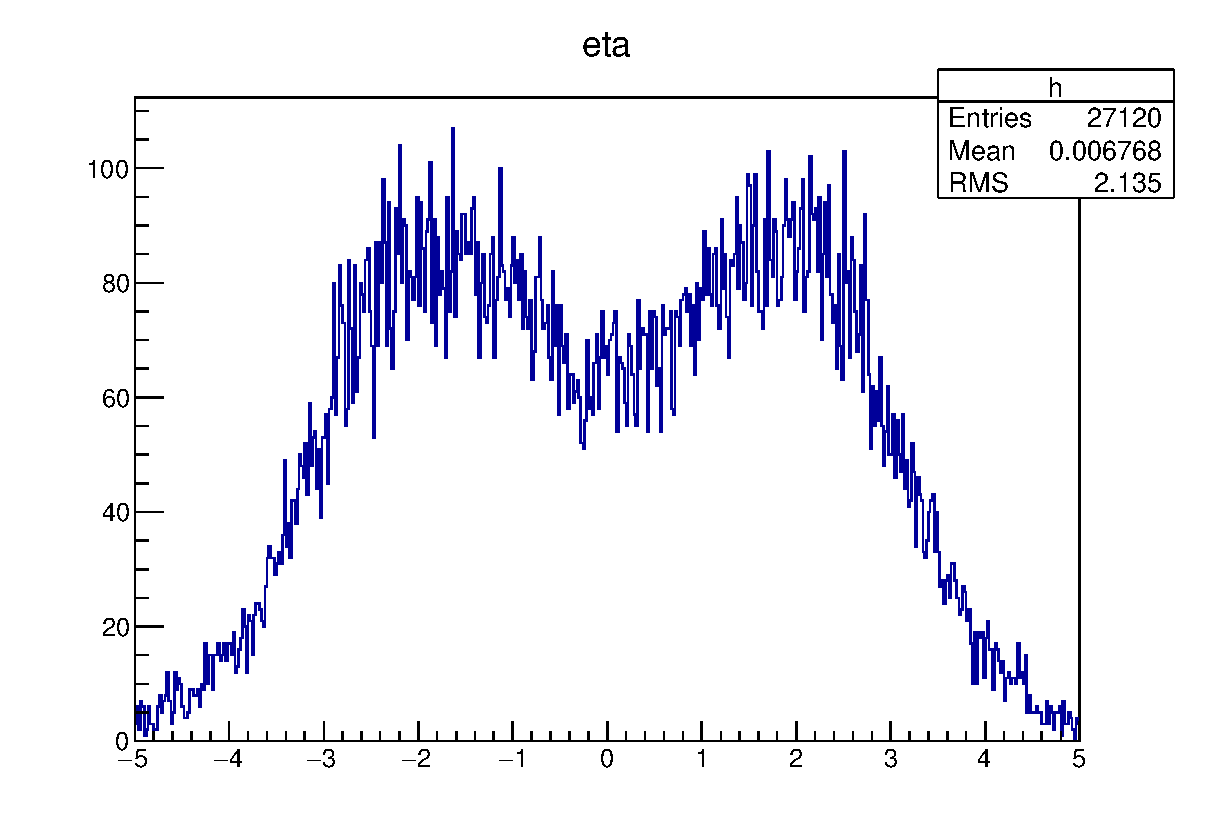
\includegraphics{../graphes/eta_gammagamma_true}
\end{figure}


\begin{figure}[h!]
  \caption{Masse invariante $e^+ e^-$ ($\simeq M_Z$) .}
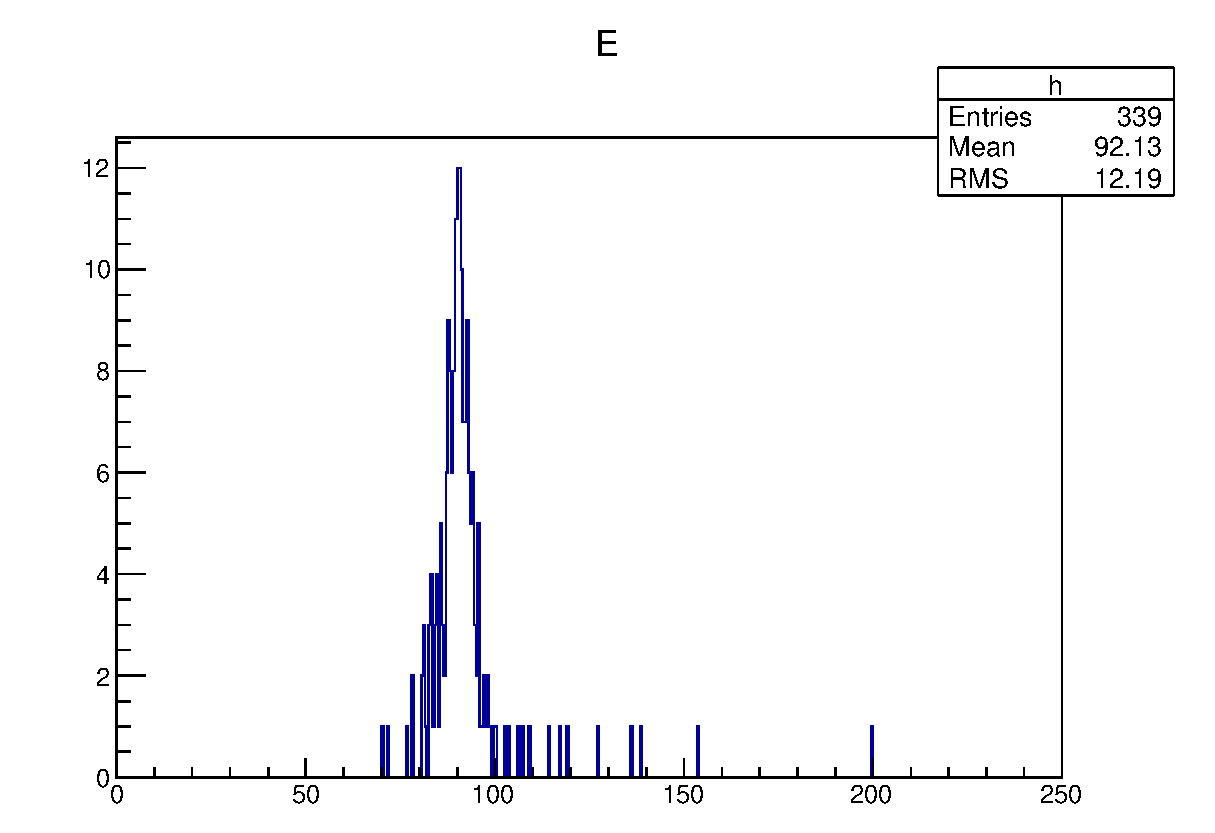
\includegraphics{../graphes/distrib_mee}
\end{figure}

\begin{figure}[h!]
  \caption{$M_{\gamma \gamma}$ avec bruit ($\sim$ 310 000 paires tight) et fit exp sur la plage 100-150 GeV }
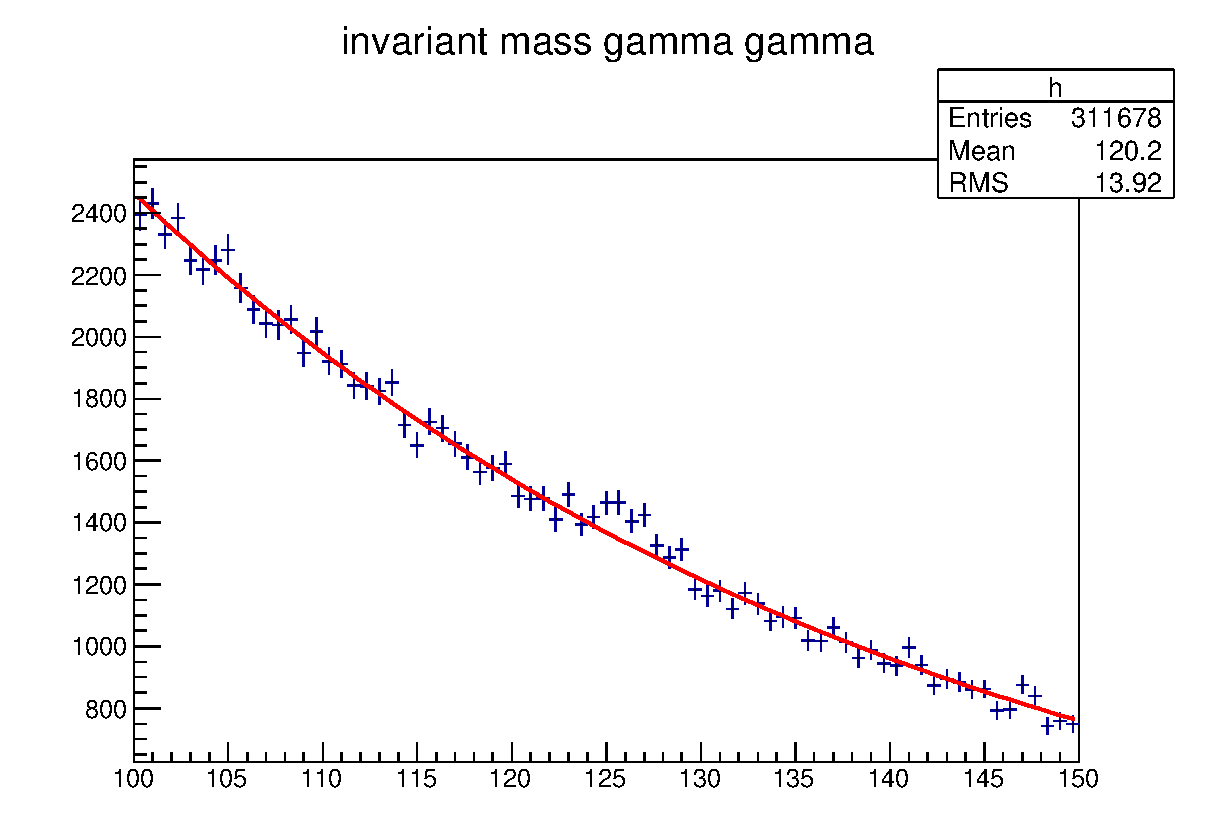
\includegraphics{../graphes/mgg_avec_bruit}
\end{figure}

\begin{figure}[h!]
  \caption{$M_{\gamma \gamma}$ - fit background.}
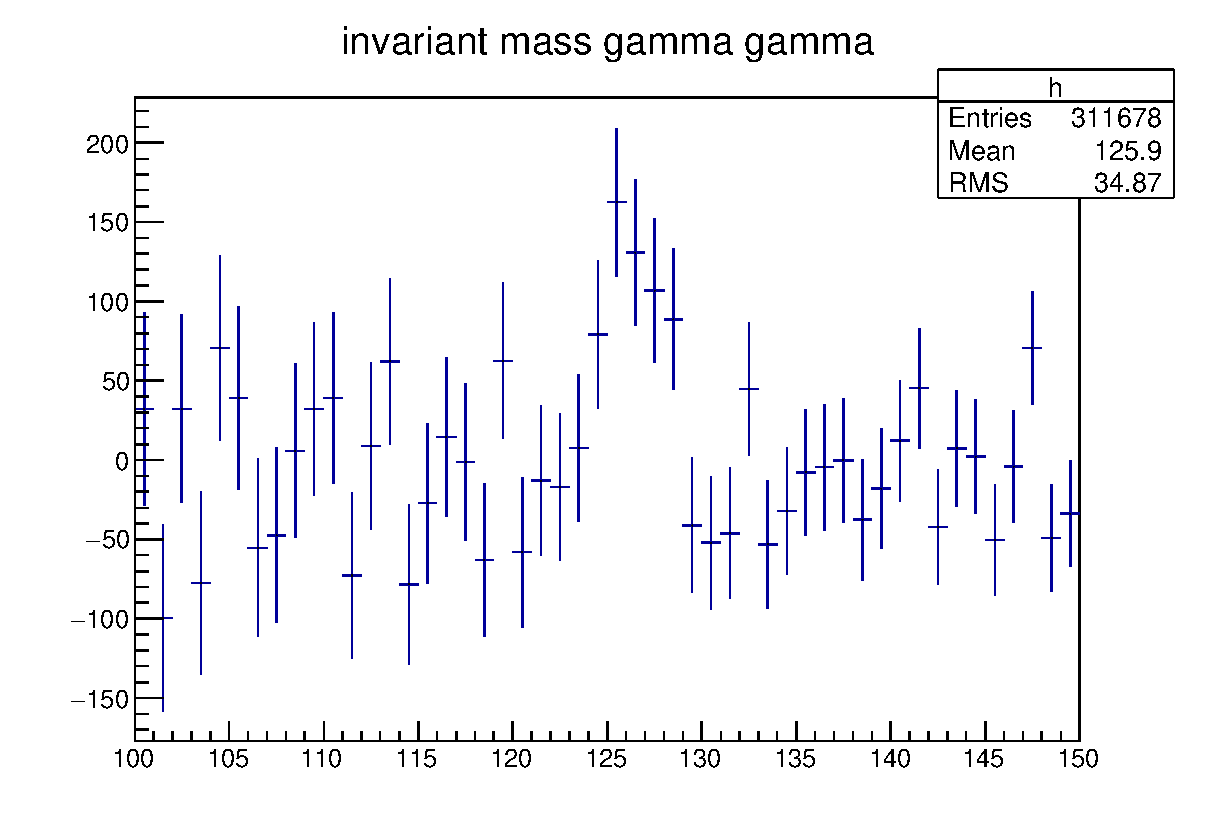
\includegraphics{../graphes/mgg_minus_bckgrnd_50}
\end{figure}

\end{document}
